\subsection{The Current State of ECDAR}\label{sub:the-current-state-of-ecdar} %This was written quite fastly ;)
This section will go over the ECDAR tool, to further illustrate the intent of ECDAR and how far it has been developed. The GUI of ECDAR 2.3.3 can be seen in \autoref{fig:ECDAR-gui}.

The GUI is split up into three vertical panes, as seen in \autoref{fig:ECDAR-gui}. The different components in the project are listed in the project pane to the left, the currently selected component is shown in the editor pane in the middle, and the queries are found in the query pane to the right.
The GUI also has a top bar, from where it is possible to open a project, hide panes, choose engine options, and more.  
Additionally, the GUI has a bar in the bottom of the view. Here, errors and warnings are supposed to be displayed.

\begin{figure}[H]
    \centering
    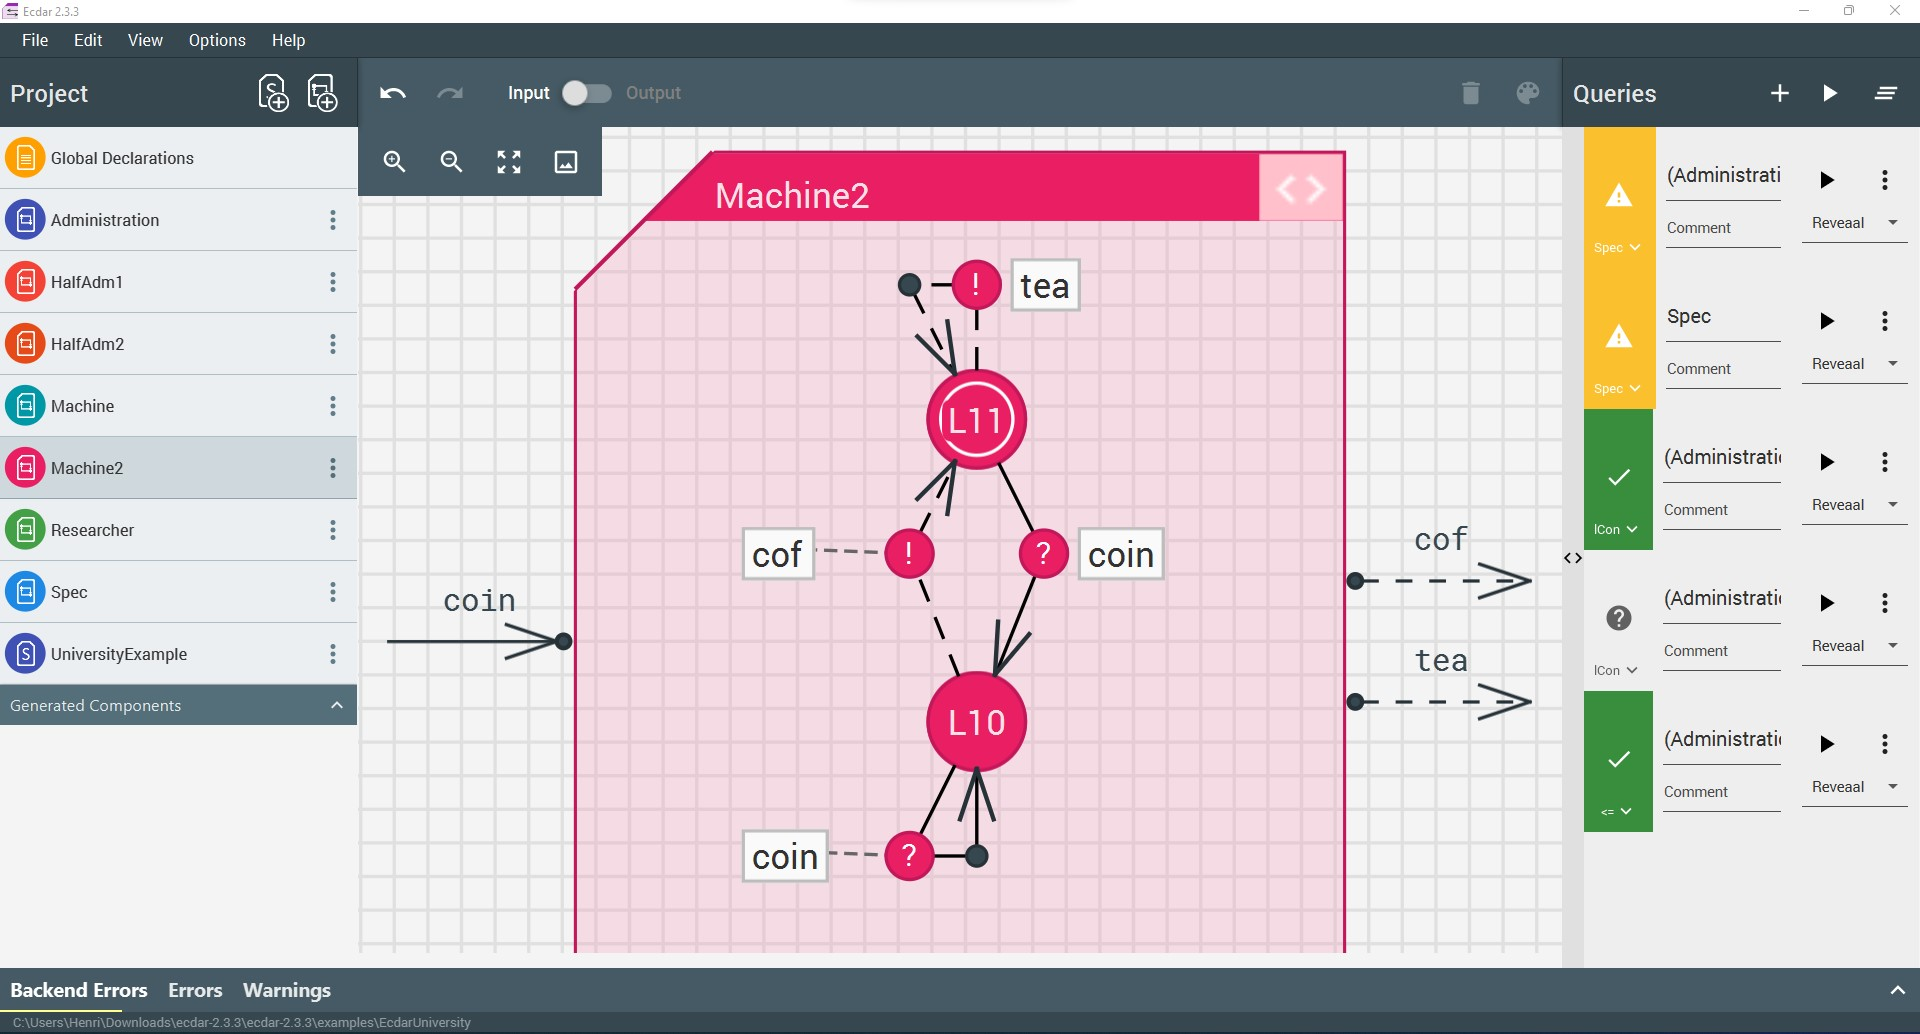
\includegraphics[width=1\textwidth]{common/figures/ecdar-overview.jpg}
    \caption{A screenshot of the ECDAR GUI of the latest version (ECDAR 2.3.3 released on 2022-09-08) \cite{ECDARNETreleasenotes}.}
    \label{fig:ECDAR-gui}
\end{figure}

\subsubsection{Project Pane}
The project pane has a header containing two buttons for creating new components and systems. The components are listed alphabetically just below this header. 
In the bottom of the pane, there is a section for automatically generated components.

\subsubsection{Editor Pane}
In \autoref{fig:ECDAR-gui}, the component \textit{Machine2} is selected. Therefore, it is shown in the editor pane. The editor pane can display one or four components at a time.
In the editor pane, it is possible to modify the components, e.g., by adding and removing transitions and locations.


\textit{Machine2} is a model of a coffee machine. The accepted input is shown on the left side of the component as a solid arrow pointing towards the component, here the input is \texttt{coin}. On the right side, the output from the coffee machine, namely \texttt{cof} and \texttt{tea}, is illustrated with dashed arrows pointing away from the component. 
Inside the component, the model is composed of locations in the shape of big circles, and transitions marked by arrows between the locations. The initial location, \texttt{L11}, is marked by a white circle around the text.
The two different types of transitions (output and input) are distinguishable through the type of line (dashed or solid), and through the symbols in the small circles on the arrows. The exclamation mark indicates an output, e.g., tea on the transition from \texttt{L11} to itself in the top of the model. A question mark, on the other hand, indicates an input. An example of that is the transition from \texttt{L11} to \texttt{L10}.

Apart from the mentioned features, it is also possible to add guards and updates, as well as invariants by right-clicking the transitions and locations, respectively. An example of a guard is provided in \autoref{fig:ECDAR-guard} as a circle containing the less-than symbol with an associated text box in which the actual guard is added and can be edited. 
An update is represented in a similar manner, but with the equals symbol in the small circle. This is shown in \autoref{fig:ECDAR-guard} on the transition from \texttt{L5} to \texttt{L4}.

\begin{figure}[H]
    \centering
    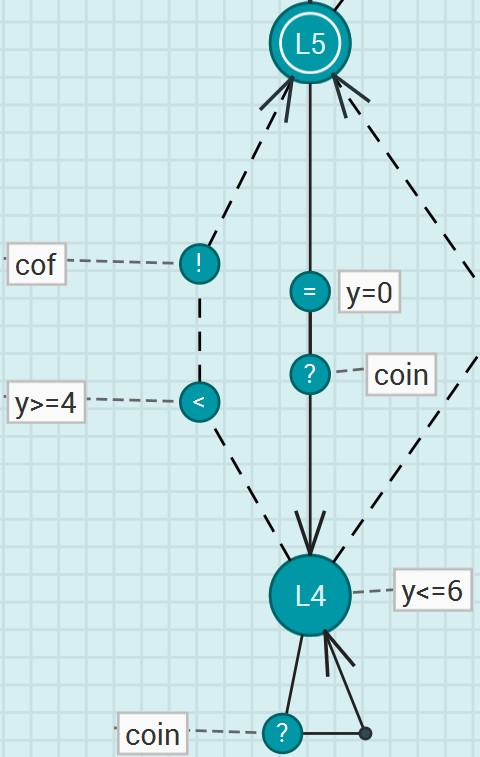
\includegraphics[width=0.3\textwidth]{common/figures/ecdar-guards.jpg}
    \caption{A screenshot of a model containing both guards, updates, and invariants.}
    \label{fig:ECDAR-guard}
\end{figure}

An example of an invariant can be seen in \autoref{fig:ECDAR-guard} as a text box with a dashed line connecting it to location \texttt{L4}. The invariant is edited in a manner similar to that of the guards and updates. 


\subsubsection{Query Pane}
The query pane has a top bar in which a query can be added using the plus symbol and by clicking the play symbol all queries can be run at the same time. Additionally, the icon next to the play icon will clear all queries. Queries are the operations that can be performed on the components. There are different types of queries and these can be seen in \autoref{tab:querytypes}. 

\begin{table}[H]
\begin{tabular}{ll}
\textbf{Query Type} & \textbf{Description} \\
reachability [E$<>$]     & x                    \\
refinement [$\leq$]      & x                    \\
quotient [\textbackslash]& x                    \\
specification [Spec]     & x                    \\
implementation [Imp]     & x                    \\
consistency [lCon]       & x                    \\
global-consistency [gCon]& x                    \\
bisim [bsim]             & x                    \\
get-component [get]      & x                    \\
\end{tabular}
\caption{\label{tab:querytypes}Table describing the different query types. The functionality of every query type is currently not implemented.}
\end{table}

Below the top bar in the query pane all the added queries can be seen. A query consists of a query request specified in the text-field, a query type chosen using the drop-down underneath the icon, and a backend engine. 
Queries are sent to one of the two engines, which can be selected in the drop-down menu to the right of a query. 
\begin{figure}[H]
    \centering
    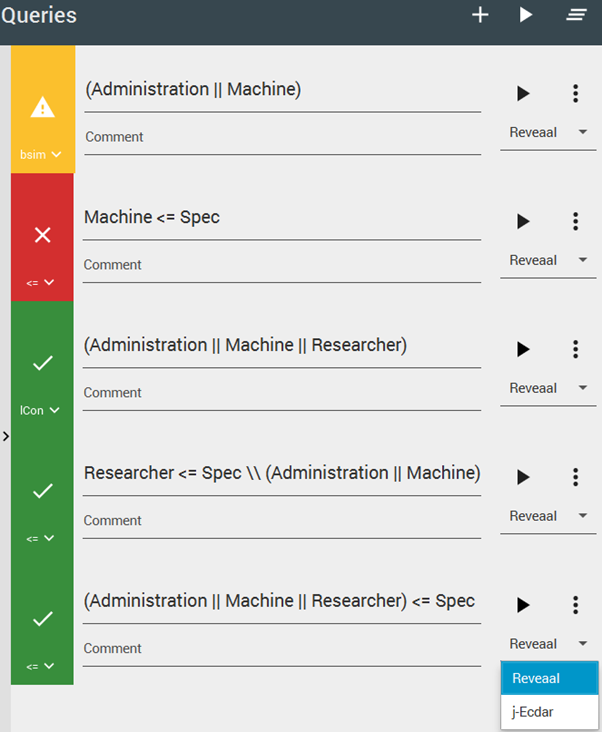
\includegraphics[width=0.6\textwidth]{common/figures/right-panel.png}
    \caption{A screenshot of the query pane.}
    \label{fig:ECDAR-queries-panel}
\end{figure}

In order to send the queries to be checked by one of the engines, the button with the \say{play} icon must be pressed.
Afterwards the result can be viewed on the left side of the pane in the form of an icon and a color.
A run of a query can result in one of three things: A green box that indicates a successful run, a yellow box that indicates an invalid query, or a red box that indicates an error.

\autoref{fig:ECDAR-queries-panel} shows five different queries. 
The result of the first query in the query pane is an error, which means the engine could not perform the query. 
An error message can be read by placing the mouse over the icon, which can be used to troubleshoot why this error occurred.
The "Machine$<=$Spec" query was performed, but the result was unsuccessful, which means the \texttt{Machine} specification did not refine the \texttt{Spec} specification.
The three remaining queries were all successful and without errors.

The text boxes use a special syntax to specify a combination of models, operators, and specifications to be checked.


%\begin{figure}[H]
%    \centering
%    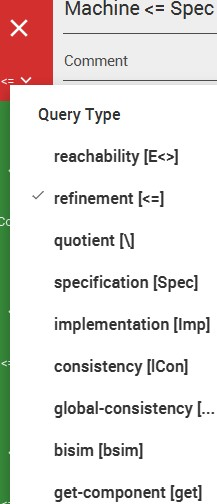
\includegraphics[width=0.25\textwidth]{common/figures/check-type.jpg}
%    \caption{A screenshot of drop-down menu with the query types.}
%    \label{fig:ECDAR-query-types}
%\end{figure}

%The type of the query to be performed is chosen in the drop-down menu underneath the icons. 
%The drop-down menu with the types of queries that can be chosen, can be seen in \autoref{fig:ECDAR-query-types}.


